\section{Project Overview}
\label{sec:outcomes}
Aegis Perception studies whether adverse-weather restoration improves both
image fidelity and object detection, and what that improvement costs on an
edge device. The experiments connect a four-weather benchmark to controlled
YOLOv8n comparisons and measurements on the original 4\,GB Jetson Nano.

\noindent\begin{minipage}{\linewidth}
\centering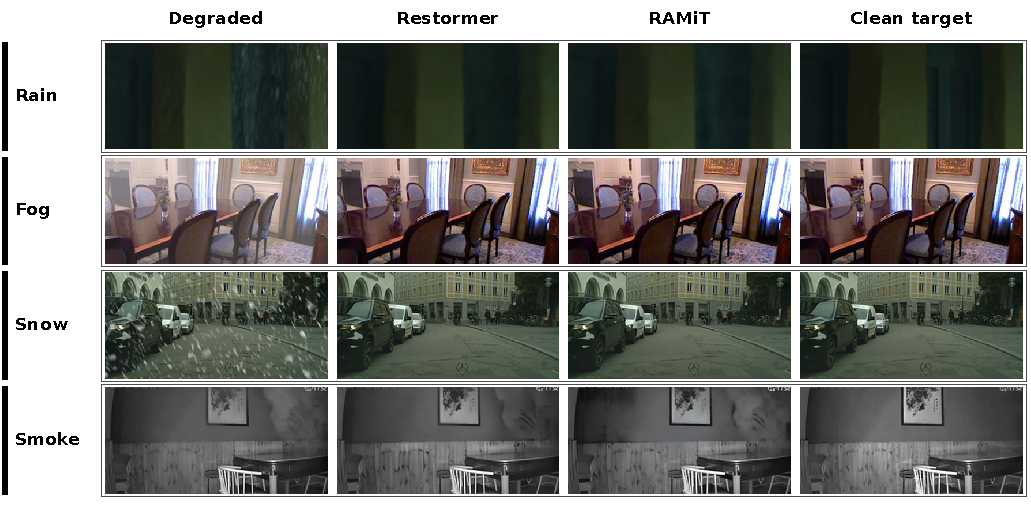
\includegraphics[width=\linewidth]{figures/weather_examples_mono.pdf}
\captionof{figure}{Four-weather restoration comparison. Each row shares one display crop; examples were fixed by sample-ID hash before score inspection. Saved predictions use native-resolution CPU FP32; the benchmark uses BF16.}
\label{fig:qual}
\end{minipage}

\medskip
\textbf{Reconstruction and detection.} Restormer leads the six-model benchmark,
but sharper-looking images do not guarantee better detection. The local pilot
improves AP; the smaller-canvas Nano cascade loses AP and throughput.

\medskip
\noindent\begin{minipage}{\linewidth}
\captionof{table}{Principal measurements. Compare raw and restored results within each experiment: the local pilot and Nano replay use different geometries and runtimes.}
\label{tab:opening-results}
\small\renewcommand{\arraystretch}{1.15}
\setlength{\fboxsep}{5pt}\setlength{\fboxrule}{.4pt}
\fbox{\begin{minipage}{\dimexpr\linewidth-2\fboxsep-2\fboxrule\relax}
\begin{tabularx}{\linewidth}{@{}p{.25\linewidth}Yp{.32\linewidth}@{}}\toprule
Experiment & Evaluation & Measured result\\\midrule
Restoration benchmark & Six models; 2,334 test pairs & Restormer: \textbf{32.58\,dB}; SSIM 0.93\\
Matched continuation & Eight ten-epoch arms & \textbf{Epoch 51 retained}\\
Local detection pilot & 72 images; $256\times448$ canvas & AP$_{50:95}$: 29.97\% $\rightarrow$ \textbf{32.86\%}\\
Nano detection & 72 images; $128\times128$ canvas & AP$_{50:95}$: 29.59\% $\rightarrow$ \textbf{14.50\%}\\
Nano labelled replay & YOLOv8n $\rightarrow$ Restormer + YOLOv8n & 6.55--7.28 $\rightarrow$ \textbf{0.61--0.62 FPS}\\
\bottomrule\end{tabularx}
\end{minipage}}
\end{minipage}

\smallskip
Six experimental phases are complete (Fig.~\ref{fig:timeline}). Their data, controls and
device measurements support the ongoing \textbf{RAMiT + YOLOv12 edge-deployment study};
end-to-end performance for this combination is not yet measured.
\clearpage
